%!TEX root = main.tex
\section{Introduction}

\subsection{Harmful Algal Blooms}
%%%%%%%%%%%%%%%%%%%%%%%%%%%%%%%%%%%%%%%%%%%
\begin{frame}{Harmful Algal Blooms}

\begin{columns}
	\column{0.5\textwidth}

	\begin{itemize}
		\item Increase in primary productivity
		\item Explosive growth of microscopic algae and cyanobacteria
		\item Toxin-producing genera
		\item Decrease biodiversity
		\item Anoxic environment
	\end{itemize}

	\column{0.5\textwidth}
	\begin{figure}
		\hspace*{-1cm}
		\vspace*{-1cm}
		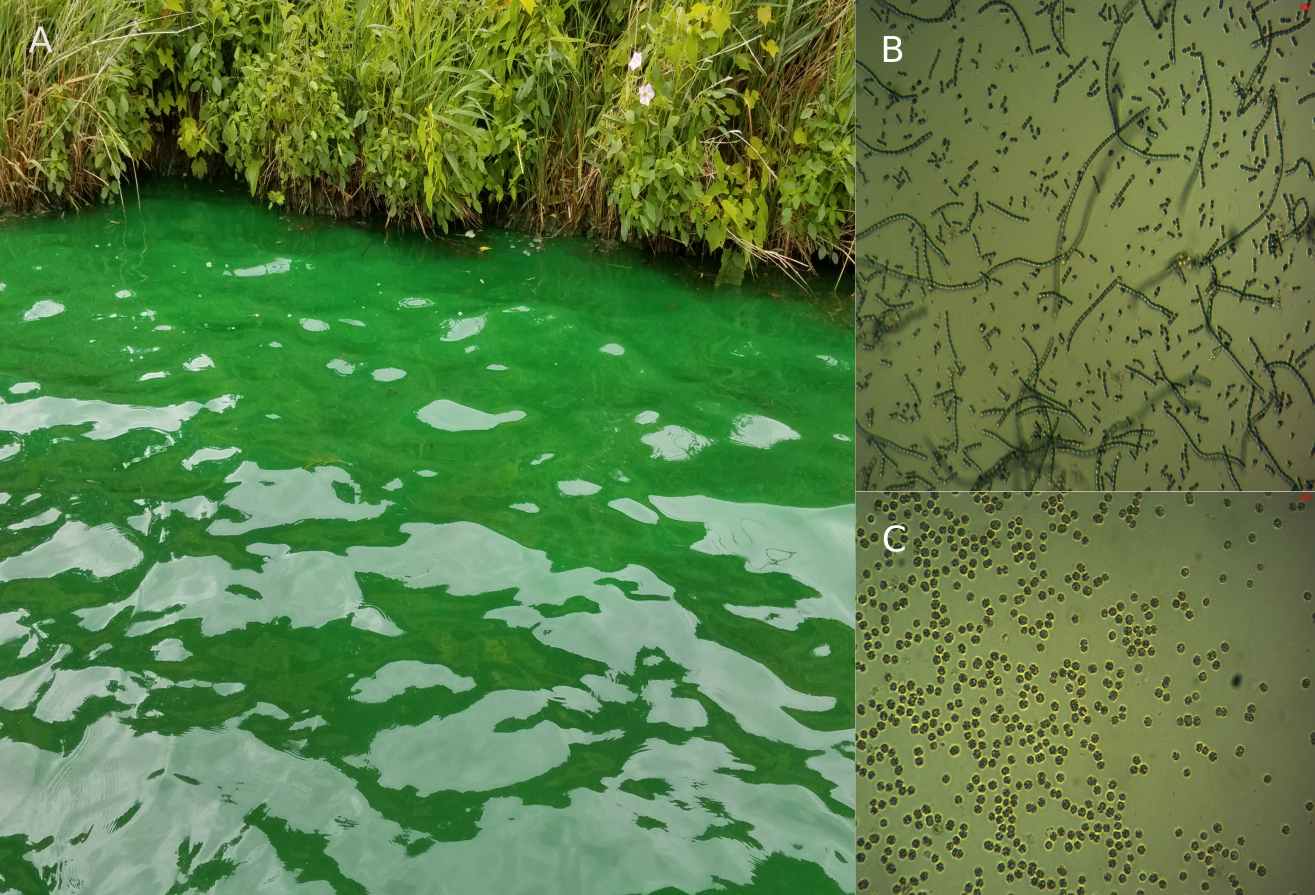
\includegraphics[width=2.4in,height=2in]{../figures/cyano.png}
	\end{figure}
\end{columns}

\end{frame}
%%%%%%%%%%%%%%%%%%%%%%%%%%%%%%%%%%%%%%%
\begin{frame}{HAB}

	\begin{itemize}
		\item Naturally occuring
		\item Exacerbate from anthropogenic causes \footcite{rastogi_cyanotoxin-microcystins:_2014}
		\item Worldwide issue
		\item Coastal environments
		\item Freshwater lakes
	\end{itemize}

\end{frame}
%%%%%%%%%%%%%%

\begin{frame}{Exposure Route}

	\begin{itemize}
		\item Direct contact
		\item Aerosols
		\item Ingestion
		\begin{itemize}
			\item Seafood/Fish 
			\item Drinking water
			\item Algal supplements
		\end{itemize}
	\end{itemize}

\end{frame}
%%%%%%%%%%%%%%
\begin{frame}{Law and Regulation}

	\begin{itemize}
		\item Safe Drinking Water Act
		\item Maximum Contaminant Level
		\begin{itemize}
			\item Regulated and enforced
		\end{itemize}
		\item Contaminant Candidate List
		\begin{itemize}
			\item ``More like guidelines''
		\end{itemize}
	\end{itemize}
\end{frame}
%%%%%%%%%%%%%%


\begin{frame}{Lake Erie 2014}
	\begin{figure}
		\centering
		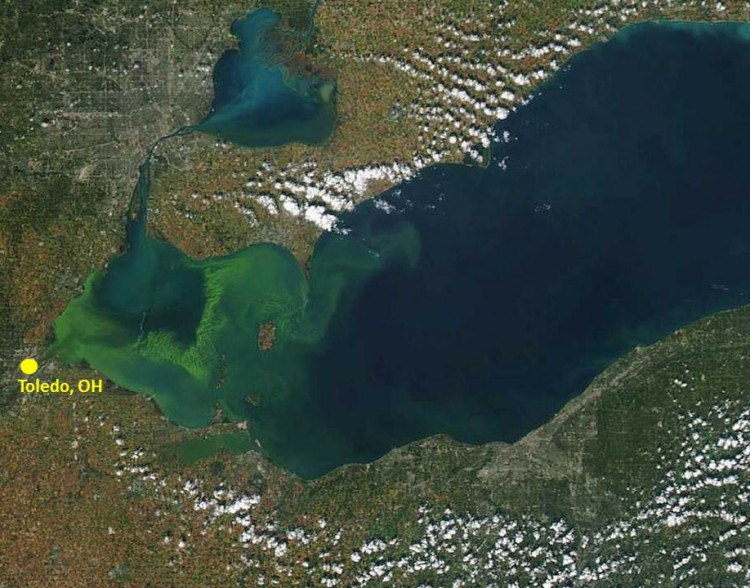
\includegraphics[scale=0.35]{erie.jpg}
	\end{figure}
\hrule
{\tiny cdn.coastalscience.noaa.gov}
\end{frame}
%%%%%%%%%%%%%%
\begin{frame}{Possible causes}
	\begin{itemize}
		\item Warmer climate 
		\item Excess nutrient inputs
			\begin{itemize}
				\item Urbanization 
				\item Agriculture 
			\end{itemize}
		\item Invasive Zebra mussels (\emph{Dreissena polymorpha})
	\end{itemize}

	<++>
\end{frame}
%%%%%%%%%%%%%%
\subsection{Cyanotoxins}
\begin{frame}{Cyanotoxins}

	\begin{itemize}
		\item Toxins
			\begin{itemize} 
				\item Microcystin and nodularin %\textsuperscript{1}
  				\item Cylindrospermopsin 
				\item Anatoxin 
				\item Saxitoxin 
				\item Produced nonribosomal polyketide synthase
			\end{itemize}
		\item Irritants
			\begin{itemize}
				\item Lipolysacharides\footcite{moore_richard_cyanobacterial_1993}
			\end{itemize}

	\end{itemize}

\end{frame}
%%%%%%%%%%%%%%

\begin{frame}{Microcystin}

\begin{columns}
	\begin{column}{0.5\textwidth}

	\begin{itemize}
		\item Cyclic peptide
		\item 1000 Da
		\item Hepatoxin and carcinogenic
		\item Inhibits protein phosphatase
		\item Diverse structures 
		\item Intra-peritoneal LD\textsubscript{50} ranging from 25-150 $\mu$g/kg  \footcite{dittmann_cyanobacterial_2012}
			\begin{itemize}
				\item Health Advisory (HA) of 4 $\mu$g/L over one day \footcite{usepa_draft_2016}
			\end{itemize}
		\item Nonribosomally polyketide synthase (NRPS)
	\end{itemize}
	\end{column}
	\begin{column}{0.3\textwidth}
\begin{figure}[ht]
	\centering
	\hspace*{-9cm}
	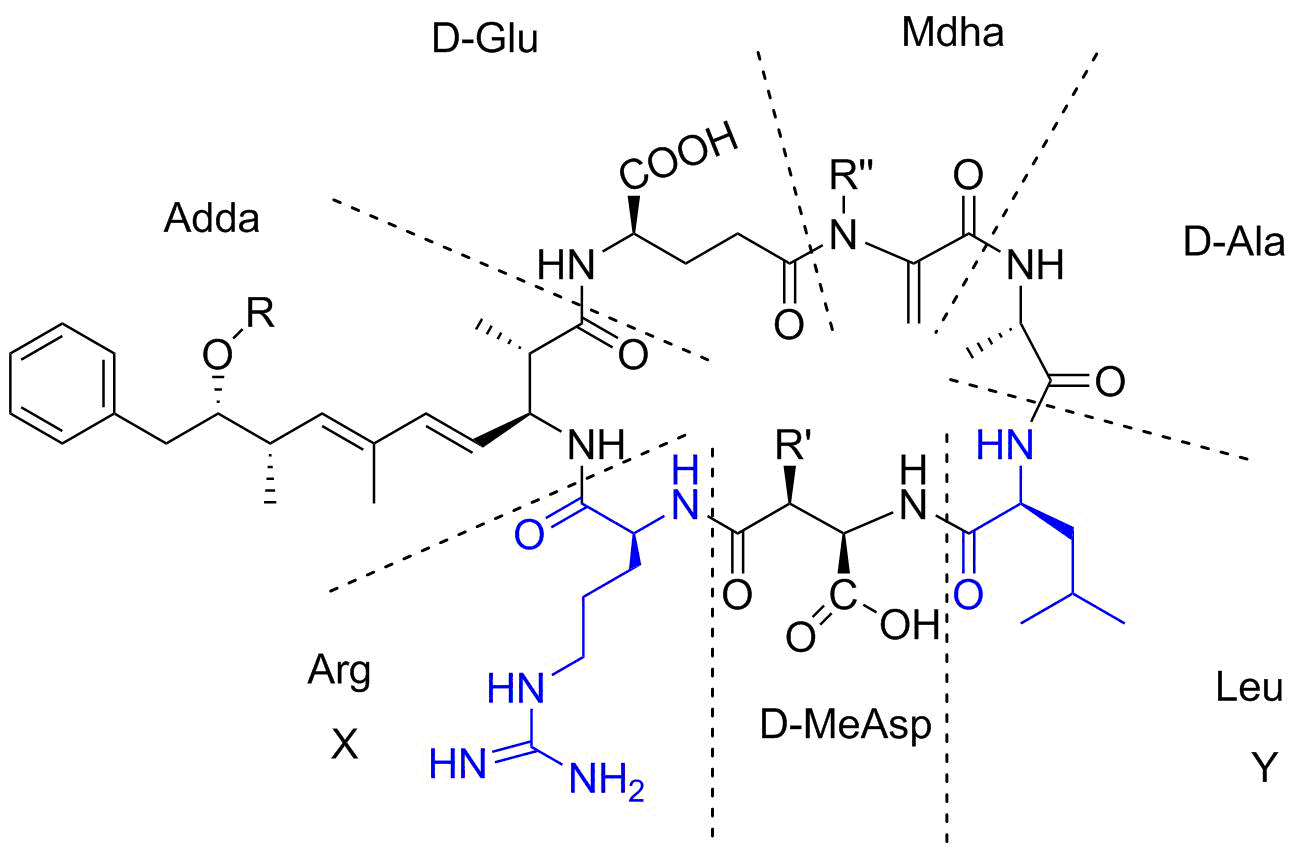
\includegraphics[width=2.2in, height=2.2in]{../figures/Microcystin-LR.png}
\end{figure}
	\end{column}
\end{columns}

\end{frame}
%%%%%%%%%%%%%%
\begin{frame}{Cylindrospermopsin}

\begin{columns}
	\column{0.5\textwidth}
	\begin{itemize}
		\item Polycyclic uracil derivative \footcite{moreira_cylindrospermopsin:_2013} 
		\item Toxicity not fully understood  \footcite{kittler_1._2014}
			\begin{itemize}
				\item Covalently binds to DNA/RNA 
				\item Inhibits protein synthesis %\textsuperscript{3} 
			\end{itemize}
		\item LD\textsubscript{50} of 150-200 $\mu$/kg over 5 days \footcite{shaw_cylindrospermopsin_2000}
			\begin{itemize}
				\item Health Advisory of 8 $\mu$g/L over one day \footcite{usepa_draft_2016}
			\end{itemize}
	\end{itemize}
	\column{0.5\textwidth}
	\begin{figure}
		\hspace*{-10cm}
		\centering
		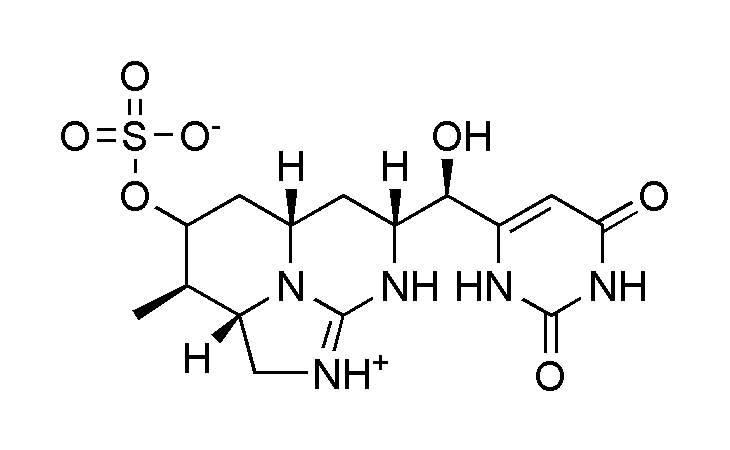
\includegraphics[width=2in]{cylindro.png}
	\end{figure}
\end{columns}
\end{frame}
%%%%%%%%%%%%%%
\begin{frame}{Anatoxin}
\begin{columns}
	\column{0.5\textwidth}
	\begin{itemize}
		\item Alkaloid 
		\item Known as Very Fast Death Factor \footcite{codd_cyanobacterial_1999} 
			\begin{itemize}
				\item Binds to acetylcholine receptor
				\item Paralysis 
				\item Respiratory failure
			\end{itemize}
		\item LD\textsubscript{50} of 300-375 $\mu$g/kg over 24 h \footcite{shaw_cylindrospermopsin_2000}
			\begin{itemize}
				\item Health Advisory of 8 $\mu$g/L over one day \textsuperscript{a} 
			\end{itemize}
	\end{itemize}
	\column{0.5\textwidth}
	\begin{figure}
		\hspace*{-10cm}
		\centering
		
\includegraphics[width=2in]{anatoxin.png}
	\end{figure}
	\hspace*{-3cm}
	\footnotesize{Test}
\end{columns}

\end{frame}
%%%%%%%%%%%%%%
\begin{frame}{Saxitoxin}
\begin{columns}
	\column{0.5\textwidth}
	\begin{itemize}
		\item Polycyclic uracil derivative \footcite{moreira_cylindrospermopsin:_2013} 
		\item Toxicity not fully understood 
			\begin{itemize}
				\item Covalently binds to DNA/RNA \footcite{kittler_1._2014} 
				\item Inhibits protein synthesis \textsuperscript{3} 
			\end{itemize}
		\item LD\textsubscript{50} of 2-10$\mu$g/kg over 24 h \footcite{shaw_cylindrospermopsin_2000}
			\begin{itemize}
				\item Health Advisory of 8 $\mu$g/L over one day \textsuperscript{a} 
			\end{itemize}
	\end{itemize}
	\column{0.5\textwidth}
	\begin{figure}
		\hspace*{-10cm}
		\centering
		
\includegraphics[width=2in]{saxitoxin.png}
	\end{figure}
\end{columns}

\end{frame}
%%%%%%%%%%%%%%
\subsection{Survey Objectives}
\begin{frame}{Objectives}
	\begin{itemize}
		\item Investigate drivers of Harmful Algal Blooms 
		\item Evaluate different techniques of detection 
		\item Do lake's with heavy urbanized watershed prone to have more cyanotoxins? 
		\item Do lake's with Zebra mussels are more at risk of cyanotoxins?
	\end{itemize}
\end{frame}
%%%%%%%%%%%%%%
\section{Survey Methods}
\subsection{Sampling}
\begin{frame}{Surveyed Lakes}

\begin{figure}
	\centering
	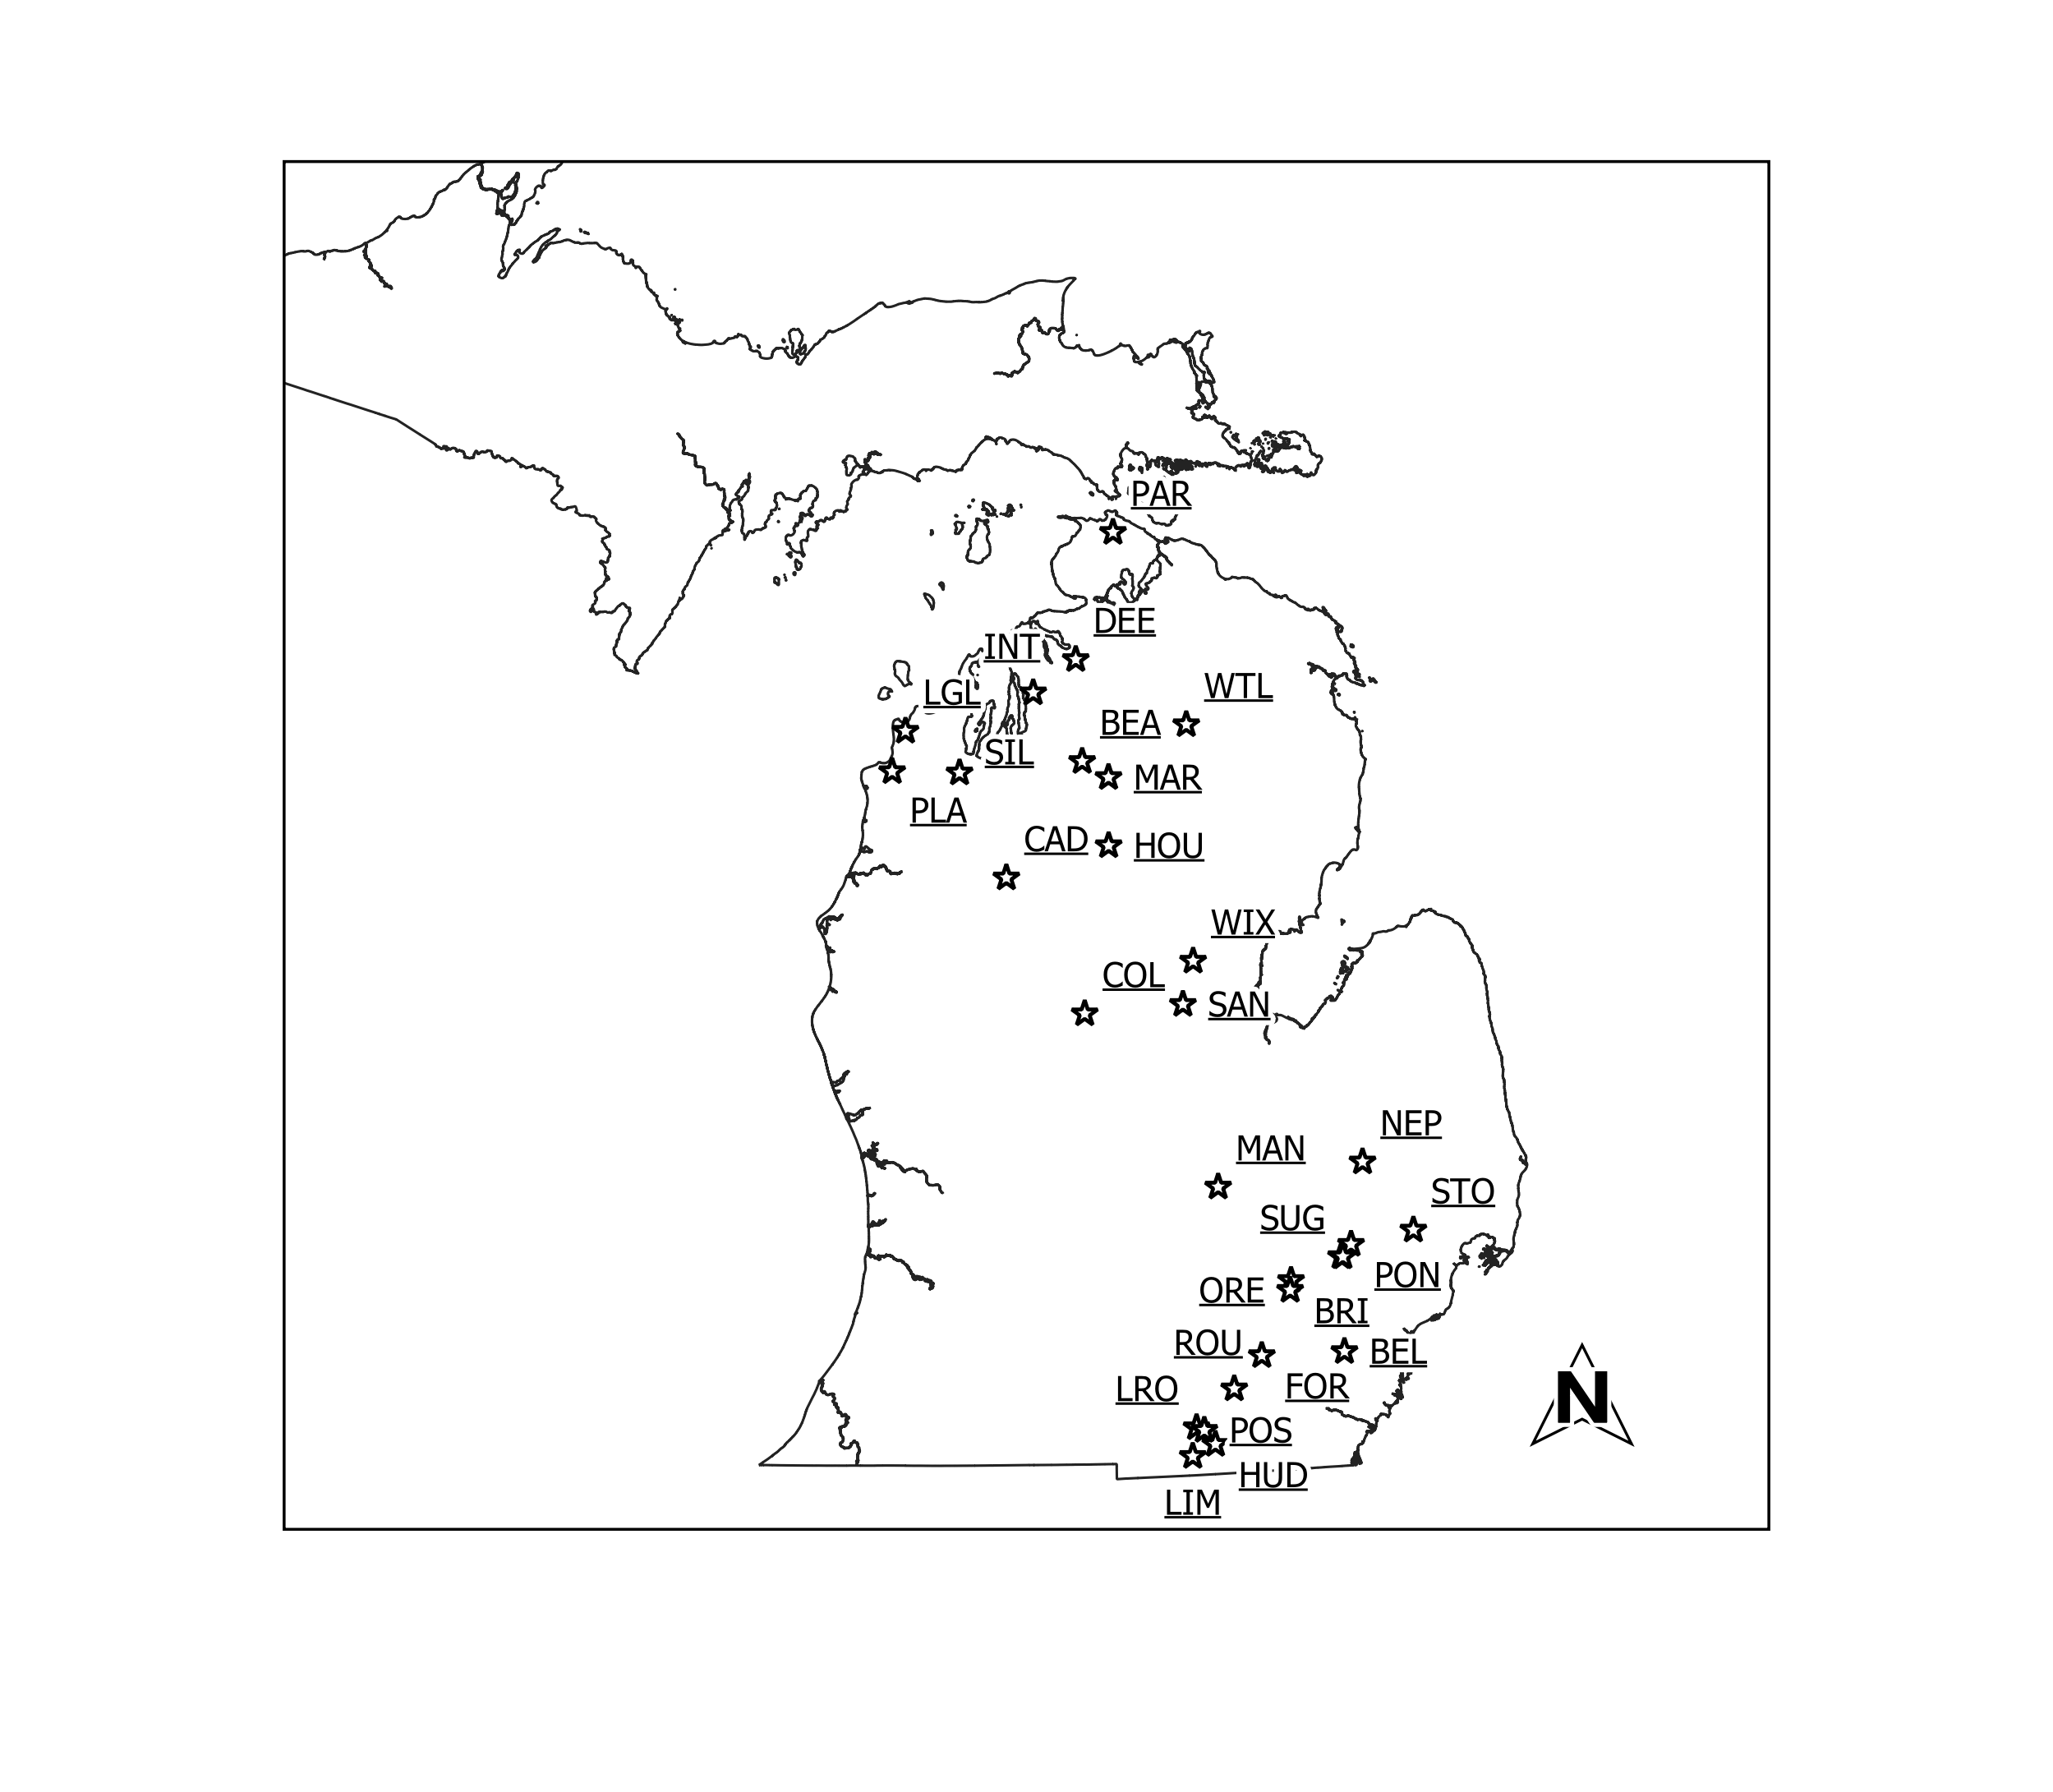
\includegraphics[width=0.8\textwidth,height=\textheight]{../figures/Overview.png}
	\caption{Sampled Lakes}
\end{figure}

\end{frame}

%%%%%%%%%%%%%%%%%%%%%%%%%%
\begin{frame}{Water Sampling}

	\begin{itemize}
		\item Sampled each lake once a month
		\item Collected water samples
			\begin{itemize}
				\item Waded in towards the center of the lake until water reaches waist height
				\item Water samples are taken roughly 10-20cm below the surface
			\end{itemize}
		\item Quickly transported back
		\item Analyzed ASAP
	\end{itemize}

\end{frame}
%%%%%%%%%%%%%%%%%%%%%%%%%%%%%
\begin{frame}
	\frametitle{Sampler}
\begin{columns}
	\column{0.5\textwidth}
	\begin{itemize}
		\item 3 PVC plates for collecting Zebra Mussels 
		\item Slotted PVC tube to hold SPATT 
		\item Installed on riparian owner's dock or on labeled floats  
		\item From July 2017 to October 2017
		\item Temperature/Light loggers 
		\item Mature Zebra mussels are collected in October
	\end{itemize}
	\column{0.5\textwidth}
	\begin{figure}
		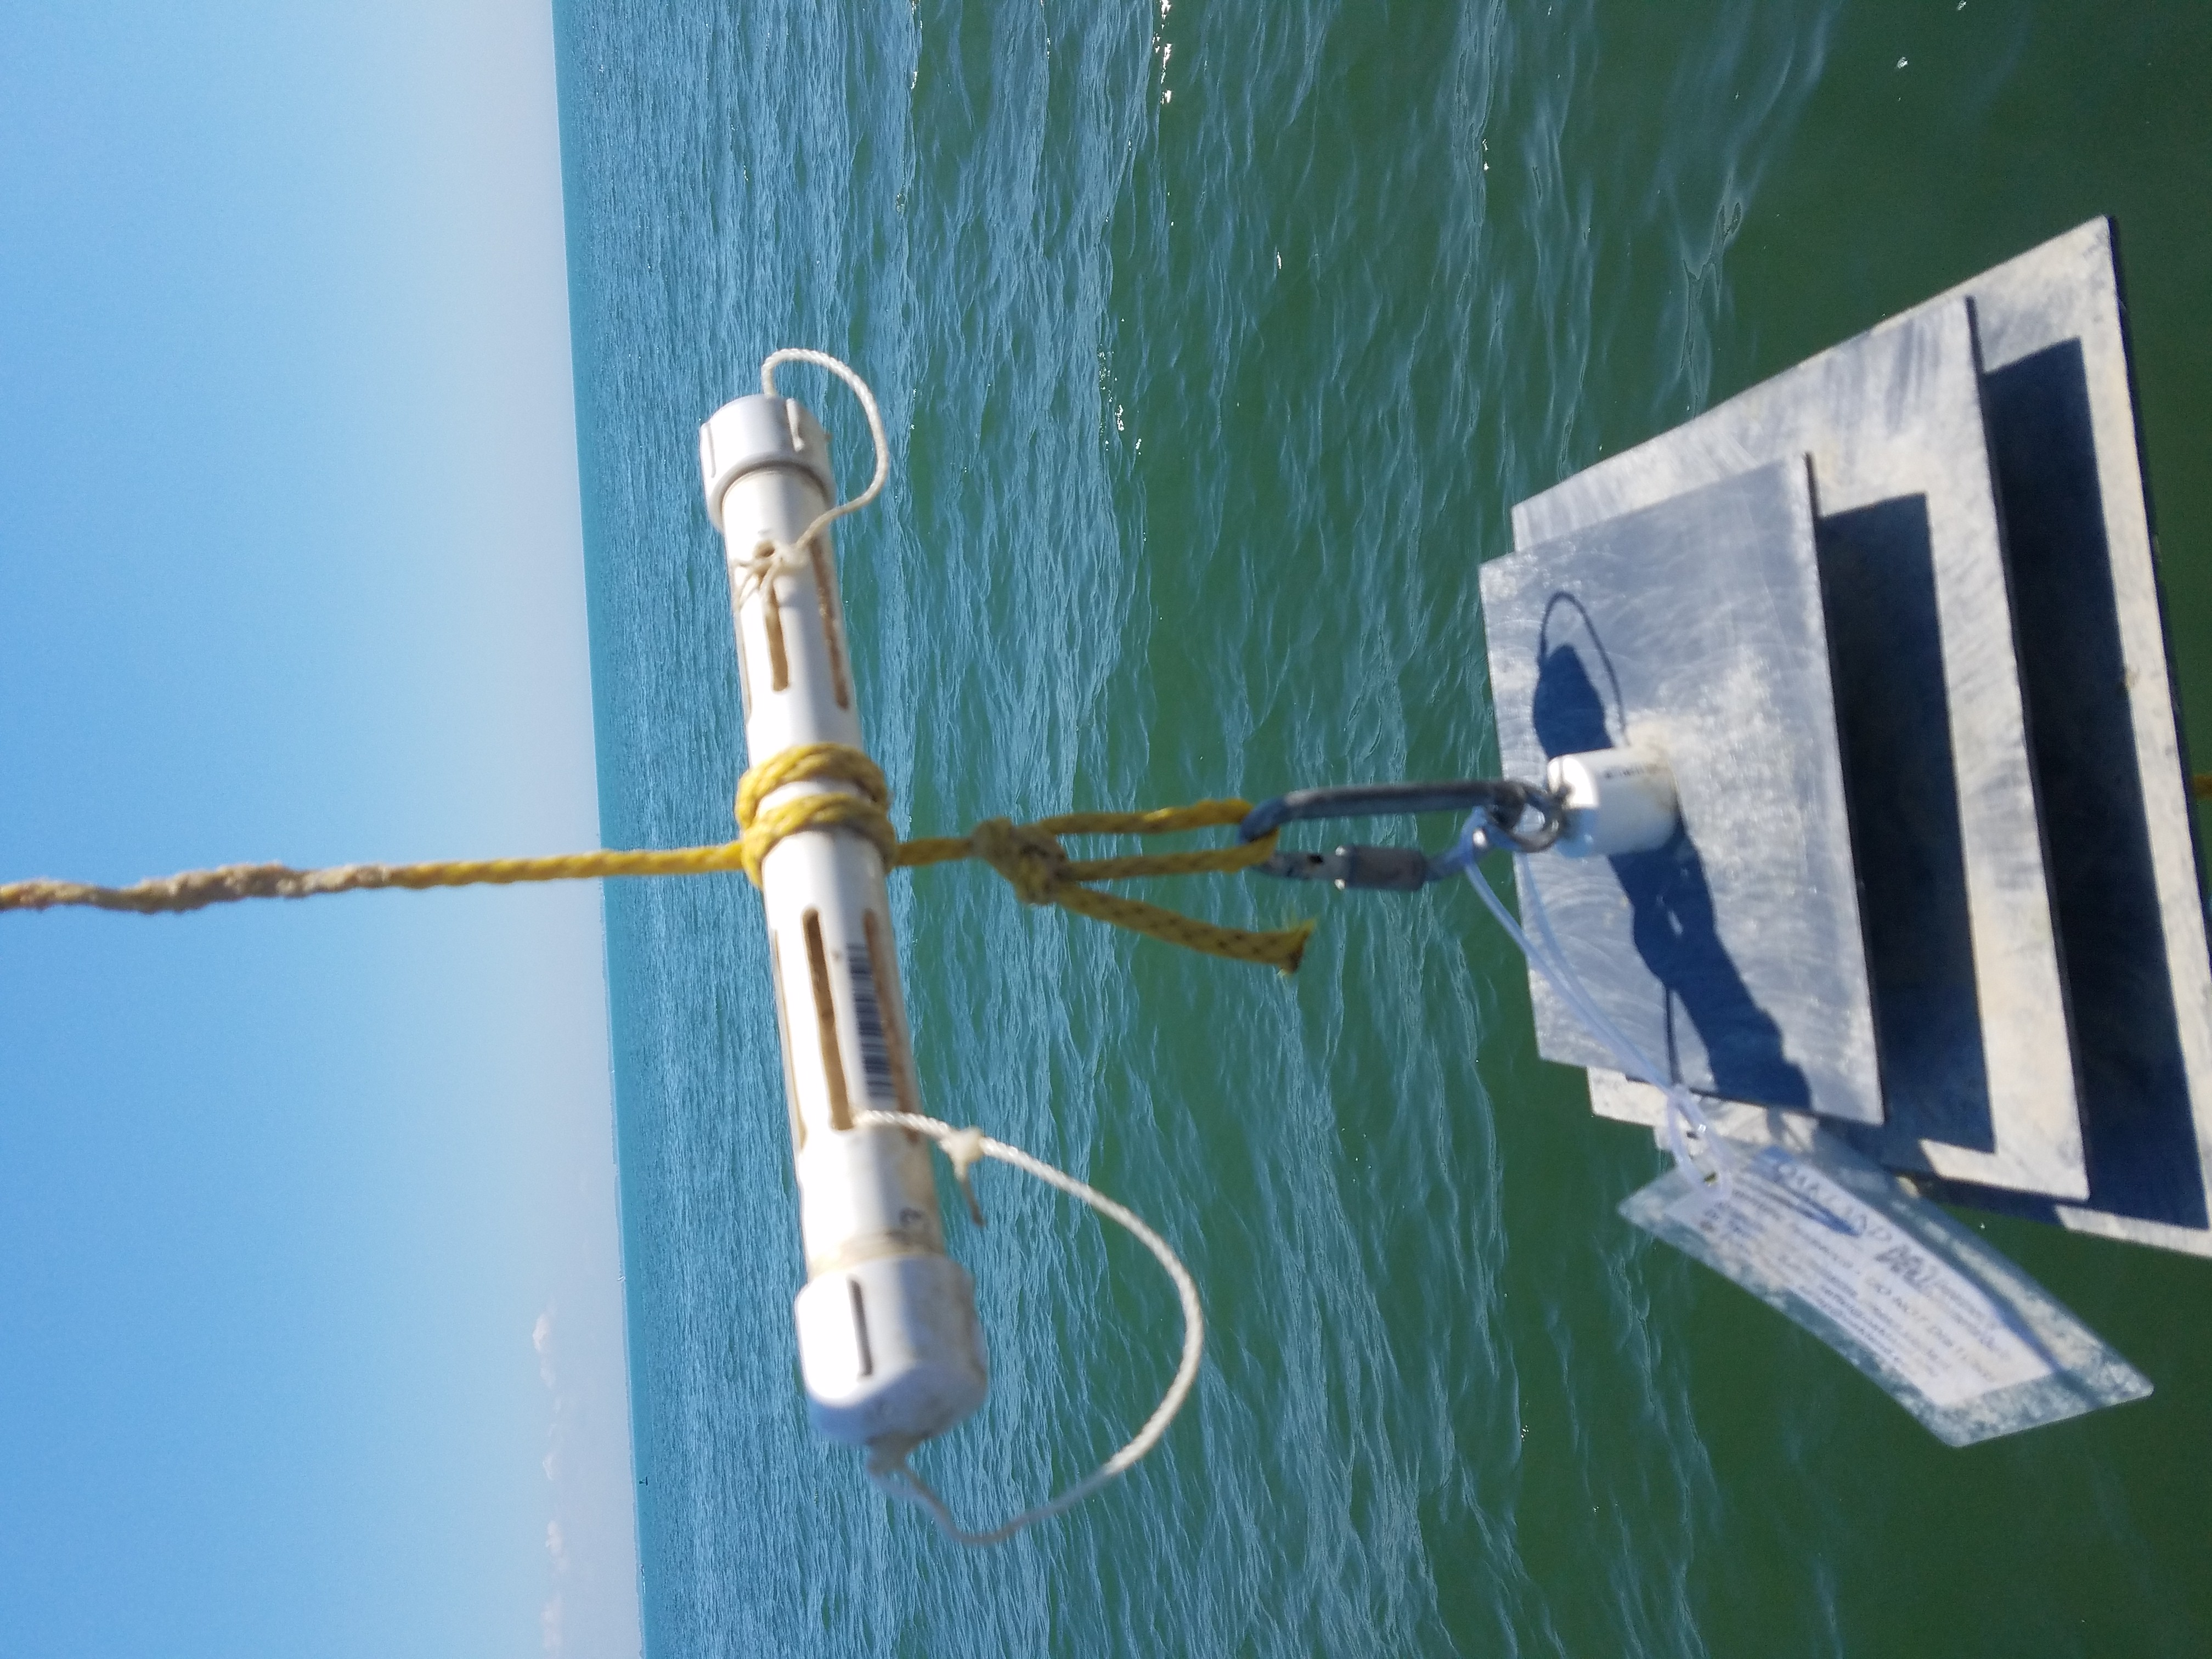
\includegraphics[width=2.3in,angle=-90]{sampler.jpg}
	\end{figure}
\end{columns}


\end{frame}



%%%%%%%%%%%%%%%%%%%%%%%%%%%%%%
\begin{frame}{SPATT}

\begin{columns}
	\column{0.5\textwidth}
	\begin{itemize}
		\item Solid phase adsorbtion toxin tracking 
		\item Dianon HP-20 
		\begin{itemize}
			\item Styrene-divinylbenzene copolymer beads
		\end{itemize} 
		
		\item Sachet filled with resin
		\item Cyanotoxin adsorb onto the resin
		\item Left for one month
	\end{itemize}

	\column{0.5\textwidth}
	\begin{figure}
		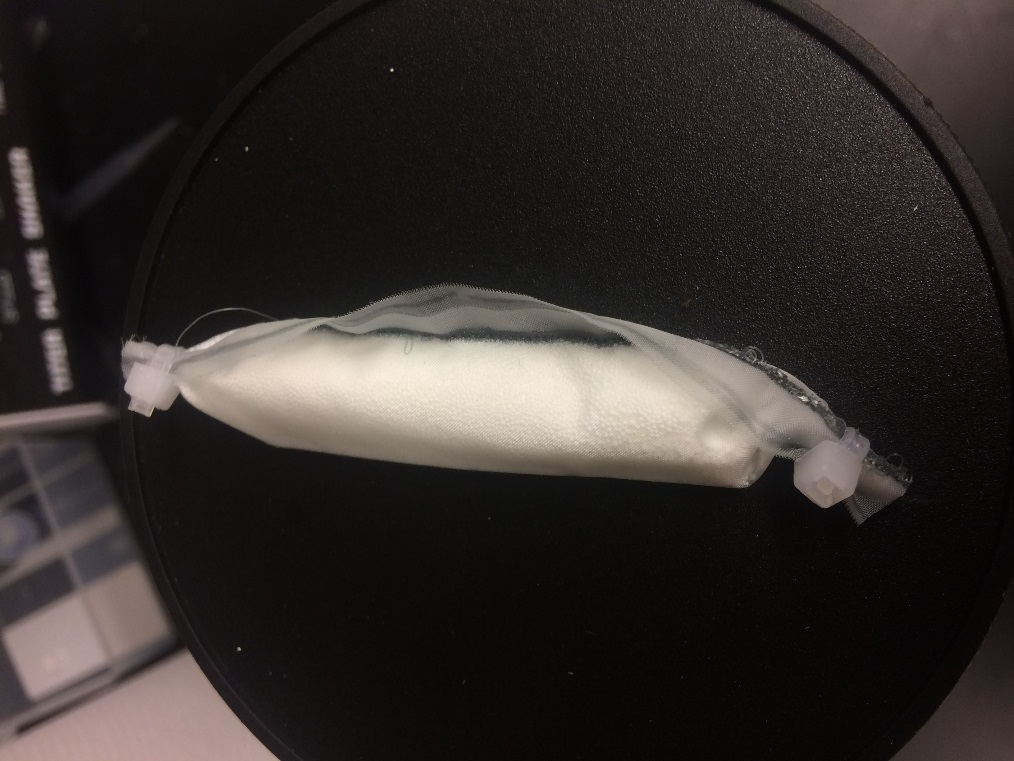
\includegraphics[width=2.3in,angle=-90]{bag.jpg}
	\end{figure}

\end{columns}

\end{frame}

%%%%%%%%%%%%%%%%%%%%%%%%%%%%%

\subsection{Chemical Analysis}

%%%%%%%%%%%%%%%%%%%%%%%%%%%%%%%
\begin{frame}{Nutrients}
	\begin{itemize}
		\item Orthophosphate-P 
		\item Nitrate+nitrite-N
		\item Ammonia-N 
		\item Total Kejdlahl nitrogen 
		\item Total Phosphorus
	\end{itemize}

	

\end{frame}

%%%%%%%%%%%%%%%%%%%%%%%%%%%%%%
\begin{frame}{LC-MS/MS}
	\begin{itemize}
		\item Freeze/Thaw
		\item Filter
	\end{itemize}

\end{frame}

%%%%%%%%%%%%%%%%%%%%%%%%%%%%%
\begin{frame}{SPATT}

	\begin{itemize}
		\item Solid phase adsorbtion toxin tracking
		\item Similar to the stationary phase
	\end{itemize}

\end{frame}
%%%%%%%%%%%%%%%%%%%%%%%%%%%%%
\begin{frame}{ELISA}

\end{frame}

\subsection{Statistical Analysis}
%%%%%%%%%%%%%%%%%%%%%%%%%%%%%
\begin{frame}{Geospatial Analysis}

\end{frame}
%%%%%%%%%%%%%%%%%%%%%%%%%%%%%
\section{Results}
\begin{frame}{Results}

\end{frame}
%%%%%%%%%%%%%%%%%%%%%%%%%%%%%
\section{Conclusion}
\begin{frame}{Conclusion}
	\begin{itemize}
		\item Most of the sampled lakes were low, with a few exceptions 
		\item Did not find any clear environmental drivers 
		\item ELISA and LC-MS/MS agree very well 
		\item Did not find association between urbanization and algal blooms 
		\item Measuring turbidity may provide a preliminary screening tool
	\end{itemize}

	
\end{frame}

%%%%%%%%%%%%%%%%%%%%%%%%%%%%%
\begin{frame}{Acknowledgment}

	\begin{itemize} 
		\item My lab team mates: Brian Spies, Andrew Herrpich, Brayden Metcalf, Mikaela Cantu and Alyssa
		\item Jason Sckrabulis, Ryan Mcwhinnie, Melissa Ostrowski, Patrick Long, James Willis
		\item Dr.David Szlag and Dr. Thomas Raffel
		\item Michigan Department Environmental Quality
		\item Oakland University and the Chemistry Department
	\end{itemize}

\end{frame}

\begin{frame}
	\frametitle{Appendix}

	

\end{frame}

<++>
